\documentclass[11pt]{book}
\usepackage[utf8]{inputenc}
\usepackage{epsfig}
\usepackage{graphicx}
\setlength{\parindent}{0pt} %junto con el de abajo
\newcommand{\forceindent}{\leavevmode{\parindent=2em\indent}} %para sangría
%\usepackage[dvips]{graphics}
%\documentclass[11pt]{book}
\usepackage[paperwidth=17cm, paperheight=22.5cm, bottom=2.5cm, right=2.5cm]{geometry}
\usepackage{amssymb,amsmath,amsthm} %paquete para símbolo matemáticos
\usepackage[spanish]{babel}
\usepackage[utf8]{inputenc} %Paquete para escribir acentos y otros símbolos directamente
\usepackage{enumerate}
\graphicspath{{Img/}} %En qué carpeta están las imágenes
\usepackage[nottoc]{tocbibind}
\usepackage{setspace}	
%\title{Tesis. Labrum = Rodete cotiloideo, rodete acetabular, labrum acetabular}
%\author{Por Mi}
%\date{2017}
\usepackage{float}
\usepackage{multirow}
\usepackage{array}


%\ 	renewcommand{\baselinestretch}{1.5}
	
\begin{document}
%\maketitle	
%-------------------------------------------------------------------------------------------
%-------------------------------------------------------------------------------------------
	\chapter{Introducción}  %---------------------------------------------------------------
	\doublespacing 
	Descripción general del tema y de cómo se tratará todo. Hacer al final


%-------------------------------------------------------------------------------------------
%-------------------------------------------------------------------------------------------
	\chapter{Análisis descriptivo}  %-------------------------------------------------------
	\doublespacing 
		%\begin{itemize}
		    %-------------------------------------------------------------------------------
			%\item Poner de qué se trata: los datos de medicina, las imágenes de medicina, y contexto
			
			%Los datos usados en la tesis son datos reales, no se incluye información personal de los pacientes para conservar la privacidad de estos. 
			
			\forceindent Antes de entrar al análisis, se dará una breve explicación de lo que son las roturas del labrum acetabular, para así comprender mejor los resultados.
			
	        \section{Contexto médico}
	        \forceindent La articulación de la cadera está formada por la cabeza femoral (superficie convexa o bola) y por el acetábulo (cavidad articular). El labrum acetabular es un borde de tejido blando, o fibrocartílago, que rodea el acetábulo. El labrum ayuda a dar estabilidad a la cadera y a proteger la unión entre la cabeza del fémur y el acetábulo. (Fuente: US San Diego Health) 
	        
	        % Imagen de la anatomía de la cadera. Poner fuente y dar explicación de la imagen
	     	\begin{figure}[h]
	     		\begin{center}
	     			\centering
	     			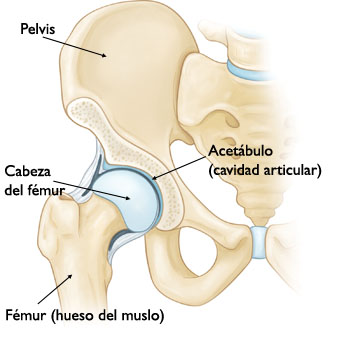
\includegraphics[scale=1.5]{cadera}
	     			\caption{Anatomía de la cadera}
	     			\label{fig:cadera}
	     		\end{center}
	     	\end{figure}
	        
	        \forceindent El labrum puede sufrir una ruptura debido a lesiones o degeneración.  Este tipo de lesiones son comunes en atletas que practican fútbol, fútbol americano, ballet, gimnasia, hockey y golf, entre otros. (Fuente: MayoClinic)
	        
	        %Imagen de tear. Poner fuente y dar explicación de la imagen
	        \begin{figure}[h]
	        	  \begin{center}
	        	     \centering
	        	     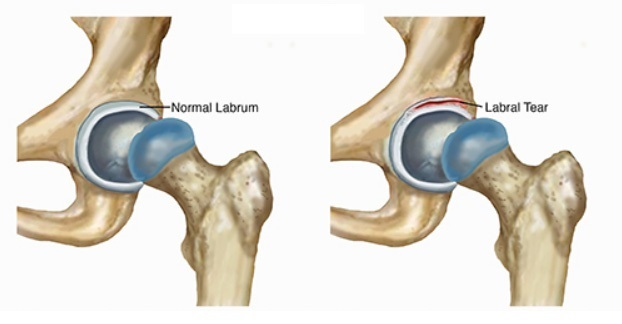
\includegraphics[scale=.6]{tear}
	        	     \caption{Lesión del labrum acetabular}
	        	     \label{fig:tear}
	        	  \end{center}
	        \end{figure}
	       
	        
	        \forceindent Para diagnosticar una lesión se puede hacer uso de radiografías, pero para obtener mayor información se usa la Resonancia Magnética (RM). En caso de que el paciente necesite intervención quirúrgica se recurre a la artroscopía de cadera, que es un procedimiento cuyo objetivo el reinsertar el labrum roto y reparar cualquier anomalía ósea que pueda tener la cadera (Fuente: Clínica Meds). --- La lectura de la RM se hace en términos de horas de un reloj de manecillas, por ejemplo, 12 a 3. ---
	        
			% Imágenes de RM y labrum (reparado). Poner fuente y dar explicación de las imágenes
	        \begin{figure}[h]
	        	\begin{center}
	        		\centering
	        		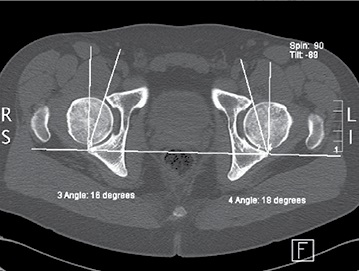
\includegraphics[scale=.6]{mrilabraltear}
	        		\caption{Resonancia magnética de cadera}
	        		\label{fig:mrilabraltear}
	        	\end{center}
	        \end{figure}			

			
	        \begin{figure}[h]
	        	\begin{center}
	        		\centering
	        		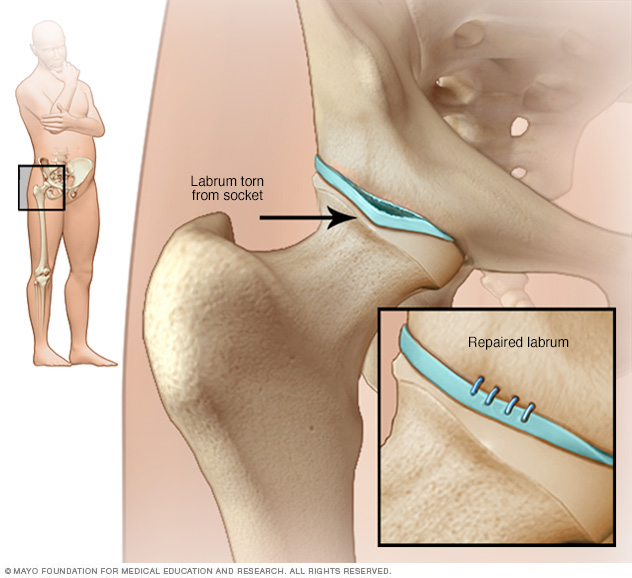
\includegraphics[scale=.2]{labrumreparado}
	        		\caption{Labrum reparado mediante artroscopía}
	        		\label{fig:labrumreparado}
	        	\end{center}
	        \end{figure}			

				
		
			
			\section{Obtención y descripción de la base de datos}
			%-------------------------------------------------------------------------------
			%\item ¿Cómo obtuve los datos? ¿Cuál es la razón y fin del análisis?
			
			\forceindent Como se mencionó al inicio del capítulo, los datos usados para el análisis son datos reales, los cuales fueron proporcionados por un médico con el fin de apoyar en el estudio. Para mantener la privacidad de los pacientes y médicos involucrados, no se incluyen nombres o datos personales, mas que la edad y el género. Los pacientes serán identificados con un ID, siendo así $paciente_{i}$, \textit{i=1,...,87}, mientras que los radiólogos serán identificados como $radiologo_{j}$, \textit{j=1,...,4}, y $cirujano$.
			
			
			
			%El problema central es el siguiente: 
			
			\forceindent En este proyecto hay cuatro radiólogos leyendo imágenes de resonancia magnética de pacientes que se quejan de dolor y se sospecha un daño en el labrum acetabular, usando el método de secuencia estándar, o SOC, por sus siglas en inglés que significan standard of care, y mediante un una nuevo método, o secuencia, denominado IDEAL. Los radiólogos interpretan la resonancia de cada paciente y, en caso de haber una lesión, la expresan como horas en un reloj de manecillas o carátula del reloj, para así conocer su localización y severidad, o extensión.
			
			\forceindent Los pacientes que efectivamente hayan sufrido una lesión del labrum son operados por medio de artroscopía, y el cirujano, quien lleve a cabo la intervención quirúrgica, evalúa el daño ``real'' y da el diagnóstico definitivo. 
			
			\forceindent Lo que se busca conocer es cuál de los dos métodos es el más acertado, es decir, por medio de cuál de los dos métodos de lectura se logra un diagnóstico más preciso de la lesión. De igual manera, determinar cuál de los cuatro radiólogos es el más acertado es sus lecturas.
			
			%\forceindent Para conocer las respuestas a estas interrogantes se hace un análisis gráfico en el que se comparan ambos métodos entre sí, y las mediciones de los cuatro radiólogos entre sí y con el diagnóstico final del cirujano, así como un análisis estadístico más profundo que incluye regresiones y pruebas de hipótesis. 
			
			\forceindent Para dar respuesta a dichas interrogantes, se hace un análisis gráfico en el que las lecturas realizadas por cada uno de los radiólogos hechas por ambos métodos, se comparan entre sí, es decir, se compara lo que dice el $radiologo_{j}$ en la lectura realizada con el método SOC versus la lectura realizada con el método IDEAL. Esto para cada uno de los pacientes. Se hace otro análisis en el que se comparan los resultados de los diagnósticos dados por los radiólogos con un método, contra el diagnóstico final del cirujano. Esto para saber la exactitud que tienen tanto cada radiólogo en su lectura, así como la exactitud de cada método o secuencia.
			
			\forceindent El análisis gráfico es sustentado por medio de un análisis utilizando regresiones y pruebas de hipótesis. AQUÍ PONER MÁS SHOW SOBRE EL ANÁLISIS ESTADÍSTICO.
			
			\forceindent Para concluir que un método es más acertado que otro para visualizar la lesión, se evalúa que tan repetibles son las lecturas entre los radiólogos para un mismo paciente, si las lecturas del mismo radiólogo son las mismas con ambos métodos, y si esos resultados son los mismos que los dictados por el cirujano después de intervenir al paciente, o si alguno subestima o sobreestima el daño real.
			
			%La pregunta es si IDEAL era mejor que SOC para visualizar el daño, y evaluar que tan repetibles son las lecturas entre radiólogos y las del mismo radiólogo con las dos secuencias.				
			
			
			
			%------------------------------------------------------------------------------	
			%\item ¿Qué datos tiene la base y cómo vienen los datos? en excel, en horas, los pacientes, etc
			
			%La base de datos proporcionada cuenta con la información anómima de 87 pacientes, para los cuales se tienen los resultados de las lecturas de sus respectivas resonancias magnéticas, interpretadas por cuatro médicos, así como el diagnóstico del médico cirujano que realizó la artroscopía en cada paciente. Esto último dato es contra el que se compararán todas las demás mediciones, ya que es "la realidad"
			
			\forceindent Los datos fueron proporcionados en una base de Excel, la cual está conformada de la siguiente manera: cada fila corresponde a un paciente diferente; las columnas incluyen la información de cada paciente, es decir, su ID, edad, género, lado donde se encuentra la lesión, si se realizó o no cirugía, el diagnóstico final del cirujano, y la lectura de la resonancia magnética realizada por cada uno de los cuatro radiólogos utilizando ambos métodos. %para los diferentes pacientes.
			
			\forceindent Como se explicó anteriormente, las lecturas de las resonancias magnéticas realizadas por cada uno de los radiólogos, así como el diagnóstico del cirujano, están expresadas como horas de un reloj de manecillas.  
			
			%-------------------------------------------------------------------------------
			%\item ¿Cómo se manipularon los datos? ¿Qué se hizo con los NA's? Conversión de reloj a círculo unitario, de horas a radianes ¿Qué se hizo con los que tenían solo una hora (12:00)? ¿Y con los que tenían dos (12:00 a 1, 2:00 a 3)?
			
			\forceindent Al contar con las lecturas de las resonancias magnéticas de cuatro diferentes radiólogos, por dos diferentes métodos, más el diagnóstico que el cirujano da una vez concluida la intervención quirúrguica, da como resultado que, por paciente, se tienen nueve diferentes datos sobre su lesión en el labrum acetabular. Para poder usar estos datos en el análisis se tuvieron que transformar. 
			
			\forceindent Algunos de los detalles a considerar para poder transformar los datos de tal forma que pudieran ser manipulados, fueron los siguientes:
			\begin{enumerate}
				\item El formato en que vienen las nueve lecturas es formato de texto, expresando la lesión como ``12 a 3''. Nótese que para una lectura se dan dos horas: la hora en la que ``empieza'' la lesión y la hora en la que ``termina'' la lesión.
				\item Hubo algunos casos en los que la lectura señalaba una lesión puntal, por ejemplo, 1200, queriendo decir las 12.
				\item En algunos pacientes se contaba con dos lecturas realizadas por el mismo radiólogo usando el mismo método. Con esto se quiere decir que el radiólogo identificó dos lesiones, o lesiones múltiples, en la misma resonancia magnética, por ejemplo, una lesión comprendida de 12 a 3 y otra de 4 a 5, o de 12 a 3 y otra solo en 400, interpretado como 4.
				\item Algunas de las horas estaban expresadas como hh30, o sea, una hora cualquiera con 30 minutos (1230 significa 12:30, por mostrar un ejemplo); lo que esto quiere decir es que la manecilla se ubica entre dos horas consecutivas, ya se entre 12 y 1, 1 y 2, 2 y 3, etcétera. Por lo que se entiende que 1230 indica que la manecilla estaría entre las 12 y la 1, lo que en un reloj de manecillas sería la hora correspondiente a 12:02:30, o 12 horas con 2 minutos con 30 segundos.
				\item En los casos en los que el radiólogo no detectó la existencia de una lesión, se señaló como $NA's$. No se ignoraron estos datos ya que son parte del estudio y de la comparación entre los dos métodos de diagnóstico, así como de las lecturas de las resonancias magnéticas realizadas por los cuatro radiólogos.
			%Para empezar, el formato en que vienen las nueve lecturas es formato de texto, expresando la lesión como 12 a 3. Segundo, en algunos pacientes se contaba con dos lecturas realizadas por el mismo radiólogo usando el mismo método. Con esto se quiere decir que el radiólogo identificó dos lesiones, o lesiones múltiples, en la misma resonancia magnética, por ejemplo, una lesión comprendida de 12 a 3 y otra de 4 a 5, o de 12 a 3 y otra solo en 400, interpretado como 4. Tercero, hubo algunos casos en los que la lectura señalaba una lesión puntal, por ejemplo, 1200, queriendo decir las 12. Cuarto, algunas de las horas estaban expresadas como hh30, o sea, una hora cualquiera con 30 minutos (1230 significa 12:30, por mostrar un ejemplo); lo que esto quiere decir es que la manecilla se ubica entre dos horas consecutivas, ya se entre 12 y 1, 1 y 2, 2 y 3, etcétera. Por lo que se entiende que 1230 indica que la manecilla estaría entre las 12 y la 1, lo que en un reloj de manecillas sería la hora correspondiente a 12:02:30, o 12 horas con 2 minutos con 30 segundos.
			\end{enumerate}	
			
			\forceindent Las lecturas que contaban con la característica del punto número 2, no se consideraron para el análisis por ser puntuales. Mientras que las que contaban con dos mediciones, como se explica en el punto 3, solo se tomó la primera lectura, ya que la mayoría de las segundas lecturas eran puntuales, y las que no lo eran mostraban una lesión casi puntual. 
			
			%-------------------------------------------------------------------------------
			%\item Definición de variables Posición y Extensión. Tabla de radianes, rangos, cómo se midieron, etc
			
			\forceindent Para poder hacer un fácil uso, manipulación y análisis de las ocho lecturas de las resonancias magnéticas y el diagnóstico dado por el cirujano, las horas en texto se convirtieron a radianes haciendo uso del círculo unitario. En este caso, las 12:00 horas es donde comienza el círculo, es decir, las 12:00 corresponde a 0 radianes.
			
			\forceindent También se definieron dos variables para facilitar el análisis. Como se explicó anteriormente, cada lectura está conformada por dos horas, una que señala el comienzo de la lesión y la otra el fin de la misma. 
			
			\forceindent Entonces cada una de las lecturas expresadas en texto fue dividida en dos variables: $X=Posicion$ y $Y=Extension$, donde 
			\begin{itemize}
				\item $X=Posicion$ se refiere a la primera hora de la lectura, y señala el punto donde comienza la lesión 
				\item $Y=Extension$ se refiere a la gravedad de la lesión, es decir, qué tan amplio es el degarre del labrum.
		    \end{itemize}
			
			\forceindent Una vez separada la lectura en dos, cada hora obtenida correspondiente a la $Posicion$ y a la $Extension$ se convirtió a radianes. 
			
			\forceindent El rango de la variable $X$, que corresponde a la $posicion$ de la herida, o donde ésta comienza, es de $(-\pi, \pi)$, donde las 12 horas equivale a $0$ radianes, las horas de 12:30 a 6 corresponden a valores positivos, mientras que las horas de 6:30 a 11 corresponden a valores negativos. (1 aquí poner pie de página señalando que la tabla de equivalencias se encuentra en el Apéndice A o 1)
			% Aquí se debe cambiar si la variable la defino de 0 a 2pi. Definit Y=|Xf-Xo|
		
			
			\forceindent Para la variable $Y$, que representa la extensión o amplitud de la lesión, el rango es de $(0, 2\pi)$ radianes. (1 aquí poner pie de página señalando que la tabla de equivalencias se encuentra en el Apéndice A o 1)
			
			\forceindent La división de la lectura en las variables mencionadas, así como la transformación que se hizo de éstas a radianes, se hizo por paciente para cada una de los ocho diagnósticos realizados por los radiólogos, y para el diagnóstico del cirujano. 
			
			\forceindent Tómese el siguiente caso como ejemplo para que quede más claro el procedimiento que se llevó a cabo: el paciente con $ID = 1$ fue sometido a una artroscopía de cadera debido a que el resultado de su resonancia magnética mostraba una lesión en el labrum acetabular. Las resultados las lecturas de la resonancia fueron los que se muestran a continuación:
			
    	
			\begin{table}[h]
				%\centering
				\begin{center}
				\scalebox{.75}{	
					\begin{tabular}{|c||c|c|c|c|c|c|c|c|c|}
						\hline 
						\multirow{2}{*}{ID} &
						\multirow{2}{*}{Cirujano} &
						\multicolumn{2}{c|}{Radiólogo 1}   &  
						\multicolumn{2}{c|}{Radiólogo 2} &
						\multicolumn{2}{c|}{Radiólogo 3} &
						\multicolumn{2}{c|}{Radiólogo 4} 
						\\ \cline{3-10}
						&  & IDEAL & SOC & IDEAL & SOC & IDEAL & SOC & IDEAL & SOC \\
						\hline 
						1 & 12 a 3 & 12 a 3 & 12 a 3 & 1 a 3 & 1 a 3 & 1 a 2 & 1 a 2 & 12 a 230 & 12 a 230 \\
						\hline		
					\end{tabular}
				}
				\caption{Horas}
				\label{Horas}
				\end{center}
			\end{table}
		
			Haciendo la división de cada lectura en $Posicion$ y $Extensicion$, se tienen los siguientes datos:

			\begin{table}[h]
				%\centering
				\begin{center}
				\scalebox{.76}{
					\begin{tabular}{|c||c|c|c|c|c|c|c|c|c|c|c|c|c|c|c|c|c|c|} 
						\hline
						\multirow{2}{*}{ID} &
						\multicolumn{2}{c|}{\multirow{2}{*}{Cirujano}} & 
						\multicolumn{4}{c|}{Radiólogo 1} &
						\multicolumn{4}{c|}{Radiólogo 2} &
						\multicolumn{4}{c|}{Radiólogo 3} &
						\multicolumn{4}{c|}{Radiólogo 4} 
						\\ \cline{4-19} 
						& %espacio para id
						\multicolumn{2}{c|}{} & %columnas para cirujano
						\multicolumn{2}{c|}{IDEAL} & \multicolumn{2}{c|}{SOC} & %columnas para Rad 1
						\multicolumn{2}{c|}{IDEAL} & \multicolumn{2}{c|}{SOC} & %columnas para Rad 2
						\multicolumn{2}{c|}{IDEAL} & \multicolumn{2}{c|}{SOC} & %columnas para Rad 3
						\multicolumn{2}{c|}{IDEAL} & \multicolumn{2}{c|}{SOC}  %columnas para Rad 4
						\\ \hline 
						1 & 
						12 & 3 & %cirujano
						12 & 3 & 12 & 3 & %rad 1
						1 & 3 & 1 & 3 & %rad 2
						1 & 2 & 1 & 2 & %rad3
						12 & 230 & 12 & 230	%rad4
						\\ \hline				
					\end{tabular}
				}
				\caption{Dividido}
				\label{Dividido}
				\end{center}
			\end{table}	
			
			Una vez realizada la división, se procede a la transformación de cada hora a radianes. La tabla siguiente muestra los resultados:
			
			\begin{table}[h]
				\begin{center}
				%\centering
				\scalebox{.6}{
					\begin{tabular}{|c||c|c|c|c|c|c|c|c|c|c|c|c|c|c|c|c|c|c|} 
						\hline
						\multirow{2}{*}{ID} &
						\multicolumn{2}{c|}{\multirow{3}{*}{Cirujano}} & 
						\multicolumn{4}{c|}{Radiólogo 1} &
						\multicolumn{4}{c|}{Radiólogo 2} &
						\multicolumn{4}{c|}{Radiólogo 3} &
						\multicolumn{4}{c|}{Radiólogo 4} 
						\\ \cline{4-19} 
						& %espacio para id
						\multicolumn{2}{c|}{} & %columnas para cirujano
						\multicolumn{2}{c|}{IDEAL} & \multicolumn{2}{c|}{SOC} & %columnas para Rad 1
						\multicolumn{2}{c|}{IDEAL} & \multicolumn{2}{c|}{SOC} & %columnas para Rad 2
						\multicolumn{2}{c|}{IDEAL} & \multicolumn{2}{c|}{SOC} & %columnas para Rad 3
						\multicolumn{2}{c|}{IDEAL} & \multicolumn{2}{c|}{SOC}  %columnas para Rad 4
						\\ \cline{1-19} 
						&  %espacio para id
						12 & 3 & %cirujano
						12 & 3 & 12 & 3 & %rad 1
						1 & 3 & 1 & 3 & %rad 2
						1 & 2 & 1 & 2 & %rad3
						12 & 230 & 12 & 230	%rad4
						\\ \cline{2-19} 
						1 & 
						X & Y & %cirujano
						X & Y & %rad1 soc
						X & Y & %rad1 ideal
						X & Y & %rad2 soc
						X & Y & %rad2 ideal
						X & Y & %rad3 soc
						X & Y & %rad3 ideal
						X & Y & %rad4 soc
						X & Y  %rad4 ideal					
						\\ \cline{2-19}
						&
						0 & 1.57 &
						0 & 1.57 &
						0 & 1.57 &
						0.52 & 1.04 &
						0.52 & 1.04 &
						0.52 & 0.52 &
						0.52 & 0.52 &
						0 & 1.30 &
						0 & 1.30
						\\ \hline						
					\end{tabular}
				}
				\caption{Radianes}
				\label{Radianes} 
				\end{center}
			\end{table}
			
		
		\forceindent Una vez terminada la separación de las horas y la conversión de estas a radianes, la base se exportó a R para hacer el análisis. 
		
		%-----------------------------------------------------------------------------------
		%\item Introducir brevemente el análisis descriptivo, i.e., solo decir que mostraré varias gráficas para explicar todo
	    %\end{itemize}
			
		\forceindent El análisis se divide en dos partes: exactitud y precisión. Para cada una de las partes se utilizarán métodos diferentes. 	
			
		\forceindent Para conocer la exactitud, se lleva a cabo un análisis descriptivo, el cual se detalla en el Capítulo 3, donde se muestran de forma gráfica las variables $X$ y $Y$ mencionadas anteriormente, así como la distribución de los pacientes por edad y género.
		
		\forceindent Mientras que en el Capítulo 4 se hace una aproximación teórica, es decir, se sustenta el análisis gráfico con métodos estadísticos más avanzados. Esto para conocer la precisión de los diagnósticos.
		
			
			
			
			
		
			
%-------------------------------------------------------------------------------------------
%-------------------------------------------------------------------------------------------
	\chapter{Exactitud \\Análisis gráfico}  %-----------------------------------------------
	\doublespacing 
	*** Aquí se va a analizar la EXACTITUD
	*** Mostrar todas las gráficas y decir qué es lo que se ve en cada una		
	*** La exactitud se refiere a la localización.	
		
	\forceindent El análisis se divide en dos partes: el análisis referente a la exactitud, y el análisis de la precisión.	
	
	\forceindent Este capítulo es sobre exactitud, es decir, qué tan acertada es la lectura hecha por los radiólogos sobre la localización de la herida, comparada contra el diagóstico final dado por el cirujano después de haber realizado la artroscopía en los pacientes.
	
	\forceindent Para conocer todos los diagnósticos y las diferencias o igualdades, se hace uso de diversas gráficas, que ayudan a mostrar la infromación de forma amigable y fácil de entender, para así llegar a una conclusión sobre qué método es más acertado, así como conocer cuál de los cuatro radiólogos es el más acertado en sus lecturas.
	
	\section{Distribución de datos (definir bien el nombre del capítulo)}
	\forceindent Antes de entrar al análisis de la variable $X$, correspondiente a la $Posicion$, se mostrará cómo se distribuyen otras variables importantes, como la edad y el género de los pacientes.
	
	
	
	
	
	
	
	\begin{figure}[H]
		\begin{center}
			\centering
			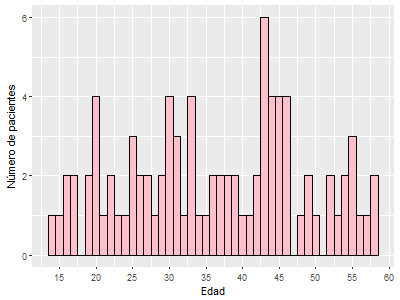
\includegraphics[scale=.8]{distribucion_edades}
			\caption{Distribución de las edades de los pacientes}
			\label{fig:edades}
		\end{center}
	\end{figure}
	
	
	
	\section{Posición}
	\forceindent Como se explicó en el capítulo anterior, las lecturas se expresan como horas de un reloj de manecillas. Cada lectura consta de dos horas, por lo que se dividieron las lecturas en dos variables. La primera hora corresponde al punto donde comienza la herida, y la segunda señala dónde termina la lesión. Ala primera hora se le denominó $Posicion$ y se le asignó la variable $X$. Esta variable es el objeto de estudio de este capítulo.
	
	\forceindent La $Posicion$ se refiere a la exactitud que cada radiólogo hace de la resonancia magnética, haciendo uso de ambos métodos: SOC e IDEAL.
	
	
	
		
		\begin{itemize}
			\item Posición
				\begin{enumerate}
					\item Gráficas para describir la base: género, lado, edad 
					\item Gráficas en las que comparo los métodos poc cada médico (son 4 por hoja): Ideal vs SOC, Ideal vs Cirujano, SOC vs Cirujano
					\item Gráficas por paciente en la que se comparan los cuatro médicos y cirujanos (son 87 gráficas y por página vienen como 20)
				\end{enumerate}	
			\item Extensión
				\begin{enumerate}
					\item Gráficas en las que compara los métodos poc cada médico (son 4 por hoja): Ideal vs SOC, Ideal vs Cirujano, SOC vs Cirujano
					\item Gráficas por paciente en la que se comparan los cuatro médicos y cirujanos (son 87 gráficas y por página vienen como 20)				
				\end{enumerate}			
		\end{itemize}
	
	
	
%-------------------------------------------------------------------------------------------
%-------------------------------------------------------------------------------------------
	\chapter{Precisión \\Aproximación teórica}  % Modelos %---------------------------------
	\doublespacing 
	Aquí se va a analizar al PRECISIÓN
	*Checar dónde comencé a usar las deltas
	Poner lo de jtter set.seed, definición del vector de deltas, vector de Métodos (con 0 y 1), y vector de Médicos (con 1, 2, 3 y 4), valores p, pruebas de hipótesis (lo del cociente o ratio -- lo tengo en la libreta el día 26 de julio), ANOVA, modelos
		\begin{itemize}
			\item Modelo1: delta ~ med
			\item Modelo2: delta ~ met
			\item Modelo3: delta ~ med + met
			\item Modelo4: delta ~ med + met + med:met
		\end{itemize}
	
	Ver lo de garantizar independencia 
	
	
%-------------------------------------------------------------------------------------------
%-------------------------------------------------------------------------------------------
	\chapter{Conclusiones}  %---------------------------------------------------------------
	\doublespacing 
	Poner aquí una recapitulación de todo lo que se hizo, y los resultados obtenidos: cúal es el método y médico más acertado, un poco de datos circulares
	
	
	
	
%-------------------------------------------------------------------------------------------
%-------------------------------------------------------------------------------------------
	\chapter{Apéndice}  %-------------------------------------------------------------------
	\doublespacing 
		\begin{itemize}
			\item Tabla de equivalencia
			
		\begin{table}[h]
			\centering
			\scalebox{1}{
			{\renewcommand{\arraystretch}{1.5}	
				\begin{tabular}{|c||c|c|}
					\hline 
					\multicolumn{1}{|c||}{Reloj} &
					\multicolumn{2}{c|}{Radianes} \\    
					\hline	
					12 & 0 & 0 \\ \hline
					1230 & $\frac{1\pi}{12}$ & 0.2618 \\ \hline
					1 & $\frac{2\pi}{12}$ & 0.5236 \\ \hline 
					130 & $\frac{3\pi}{12}$ & 0.7854 \\ \hline
					2 & $\frac{4\pi}{12}$ & 1.0472 \\ \hline
					230 & $\frac{5\pi}{12}$ & 1.3090 \\ \hline
					3 & $\frac{6\pi}{12}$ & 1.5708 \\ \hline
					330 & $\frac{7\pi}{12}$ & 1.8326 \\ \hline
					4 & $\frac{8\pi}{12}$ & 2.0944 \\ \hline
					430 & $\frac{9\pi}{12}$ & 2.3562 \\ \hline
					5 & $\frac{10\pi}{12}$ & 2.6180 \\ \hline
					530 & $\frac{11\pi}{12}$ & 2.8798 \\ \hline
					6 & $\frac{12\pi}{12}$ & 3.1416 \\ \hline
					630 & $\frac{13\pi}{12}$ & 3.4034 \\ \hline
					7 & $\frac{14\pi}{12}$ & 3.6652 \\ \hline
					730 & $\frac{15\pi}{12}$ & 3.9270 \\ \hline
					8 & $\frac{16\pi}{12}$ & 4.1889 \\ \hline
					830 & $\frac{17\pi}{12}$ & 4.4506 \\ \hline
					9 & $\frac{18\pi}{12}$ & 4.7124 \\ \hline
					930 & $\frac{19\pi}{12}$ & 4.9749 \\ \hline
					10 & $\frac{20\pi}{12}$ & 5.2360 \\ \hline
					1030 & $\frac{21\pi}{12}$ & 5.4978 \\ \hline
					11 & $\frac{22\pi}{12}$ & 5.7596 \\ \hline
					1130 & $\frac{23\pi}{12}$ & 6.0214 \\ \hline
				\end{tabular}
			}\quad
			}
		\end{table}				
			
			
		\begin{table}[h]	
			\begin{center}          
				\begin{tabular}{|c|c||c|}
					\hline 
					
					Reloj & Radianes & Radianes \\
					\hline \hline	
					6		&	$12\pi/12$	&	3.141592654	\\
					5:30	&	$11\pi/12$	&	2.879793266	\\
					5		&	$10\pi/12$	&	2.617993878	\\
					4:30	&	$9\pi/12$	&	2.35619449	\\
					4		&	$8\pi/12$	&	2.094395102	\\
					3:30	&	$7\pi/12$	&	1.832595715	\\
					3		&	$6\pi/12$	&	1.570796327	\\
					2:30	&	$5\pi/12$	&	1.308996939	\\
					2		&	$4\pi/12$	&	1.047197551	\\
					1:30	&	$3\pi/12$	&	0.785398163	\\
					1		&	$2\pi/12$	&	0.523598776	\\
					12:30	&	$\pi/12$	&	0.261799388	\\
					12		&	0			&	0		   	\\
					11:30	&	$-\pi/12$	&	-0.261799388 \\
					11		&	$-2\pi/12$	&	-0.523598776 \\
					10:30	&	$-3\pi/12$	&	-0.785398163 \\
					10		&	$-4\pi/12$	&	-1.047197551 \\
					9:30	&	$-5\pi/12$	&	-1.308996939 \\
					9		&	$-6\pi/12$	&	-1.570796327 \\
					8:30	&	$-7\pi/12$	&	-1.832595715 \\
					8		&	$-8\pi/12$	&	-2.094395102 \\
					7:30	&	$-9\pi/12$	&	-2.35619449	 \\
					7		&	$-10\pi/12$	&	-2.617993878 \\
					6:30	&	$-11\pi/12$	&	-2.879793266 \\
					6		&	$12\pi/12$	&	3.141592654	 \\		
					\hline
				\end{tabular}
			\end{center}
		\end{table}	
			
			\item Datos circulares: qué son, la función de densidad, porqué no se usaron, limitaciones por los datos, etc (checar correos de Barrios con tesis y la tesis que le mandé al inicio)
			\item Gráfica de pastelitos y una explicación
		\end{itemize}
	
	

%-------------------------------------------------------------------------------------------
%-------------------------------------------------------------------------------------------
	\chapter{Bibliografía}  %---------------------------------------------------------------
	\doublespacing 
	Fuentes, fotos, etc
	
\end{document}